% !TEX root = ./pkMain.tex
\mode*


\begin{frame}[<+->]
\mode<presentation>{\frametitle{Einleitung}}
\mode<article>{
	In der An�sthesie dosieren wir die (meisten) Medikamente entsprechend einer gemessenen oder beobachteten Wirkung. Die Zufuhr (Dosis oder Infusionrsate oder Konzentration) wird deshalb w�hrend einer An�sthesie immer wieder angepasst. Dabei kommt die \emph{zeitliche} Dimension des Dosierens ins Spiel. Diese Dimension wird in andern Bereichen der Medizin beim Dosieren weniger explizit ber�cksichtigt:
}
\begin{itemize}
\item
Das klassisches Dosieren (ausserhalb An�sthesie) ist Input basiert $=$ \enquote{Ich lege zum voraus fest, wie gross die Dosis pro KG sein muss?}
\mode<article>{\newline �ber den (exakten) zeitlichen Verlauf der Konzentration resp. Wirkung wird weniger nachgedacht.}
\begin{itemize}
	\item Dosis wird in regelm�ssigen Abst�nden verabreicht (z.B. 1x, 2x pro Tag)
	\item
	Es wird (f�lschlicherweise) angenommen, dass Dosis in eindeutiger Beziehung zur Wirkung steht.
	\item
	Die rechtzeitige Erholung von der Wirkung (\enquote{Aufwachen}) ist nicht wichtig!.
	\item
	Man nimmt an, dass bei gen�gender Dosierung der Therapieerfolg eintritt. Beurteilung des Therapieerfolgs h�ufig \enquote{bin�r} d.h. Erfolg order Nichterfolg
\end{itemize}
\end{itemize}

\mode<article>{
	Die Pharmakokinetik und Pharmakodynamik beschreiben zusammen den Prozess von der Applikation (Aufnahme) des Medikamentes bis zur Wirkung. Dies beinhaltet Aufnahme in Blut (bei oraler Applikation), zeitlicher Verlauf der Konzentration im Blut (Umverteilung, Elimination), zeitlicher Verlauf der Aufnahme und Elimination des Medikamentes in den und aus dem Wirkort sowie die Beziehung zwischen der Konzentration am Wirkort und der Wirkung.
}


\note<1>
{
\begin{itemize}
\item
Wenn ich Gewicht ber�cksichtige nicht mehr weiterdenken?
\\
Beispiel machen: 50 kg x 2 mg Propofol; 100 kg x 2 mg
\item
Was passiert mit dem Medikament nach Injektion, was passiert mit dem Medikament?
\item
Wichtig ist es die Wirkung zu beurteilen\\
Nicht Packungsprospekt = Input; Sondern, was braucht der Patient?
\item
Welche Ziele verfolgen sie? :: Schlaf, evt. schnell Einschlafen, Analgesie, Blutdruck, Herzfrequenz, schmerzfrei Aufwachen, gen�gend Atmen, Reflexe etc.
\end{itemize}
}
\infina
\end{frame}

\begin{frame}[<+->]
\mode<presentation>{\frametitle{Einleitung 2}}
\mode<article>{
	In der An�sthesie dosieren wir die (meisten) Medikamente entsprechend einer gemessenen oder beobachteten Wirkung. Die Zufuhr (Dosis oder Infusionrsate oder Konzentration) wird deshalb w�hrend einer An�sthesie immer wieder angepasst. Dabei kommt die \emph{zeitliche} Dimension des Dosierens ins Spiel. Diese Dimension wird in andern Bereichen der Medizin beim Dosieren weniger explizit ber�cksichtigt:
}
\begin{itemize}

\item
(Klassisches) Dosieren in An�sthesie: Bolus und Infusionsrate
\begin{itemize}
	\item
	Man beginnt evt. mit Bolus (adaptiert gem�ss z.B. Gewicht) oder startet mit einer Infusionrate (wieviel?)
	\item
	Erwartung: Infusionsrate proportional zur Wirkung. (ist nur im SS so!)
	\item
	Situatives dosieren $=$ Anpassen Dosis/Infusionsrate entsprechend der ben\"otigten Wirkung.
	\item
	Auch angepasste Dosis/Infusionsrate NICHT in eindeutiger Beziehung zu Wirkung!
\end{itemize}

\end{itemize}


\note<1>
{
\begin{itemize}
\item
.
\end{itemize}
}
\infina
\end{frame}





\mode<presentation>{
\begin{frame}
	\begin{center}
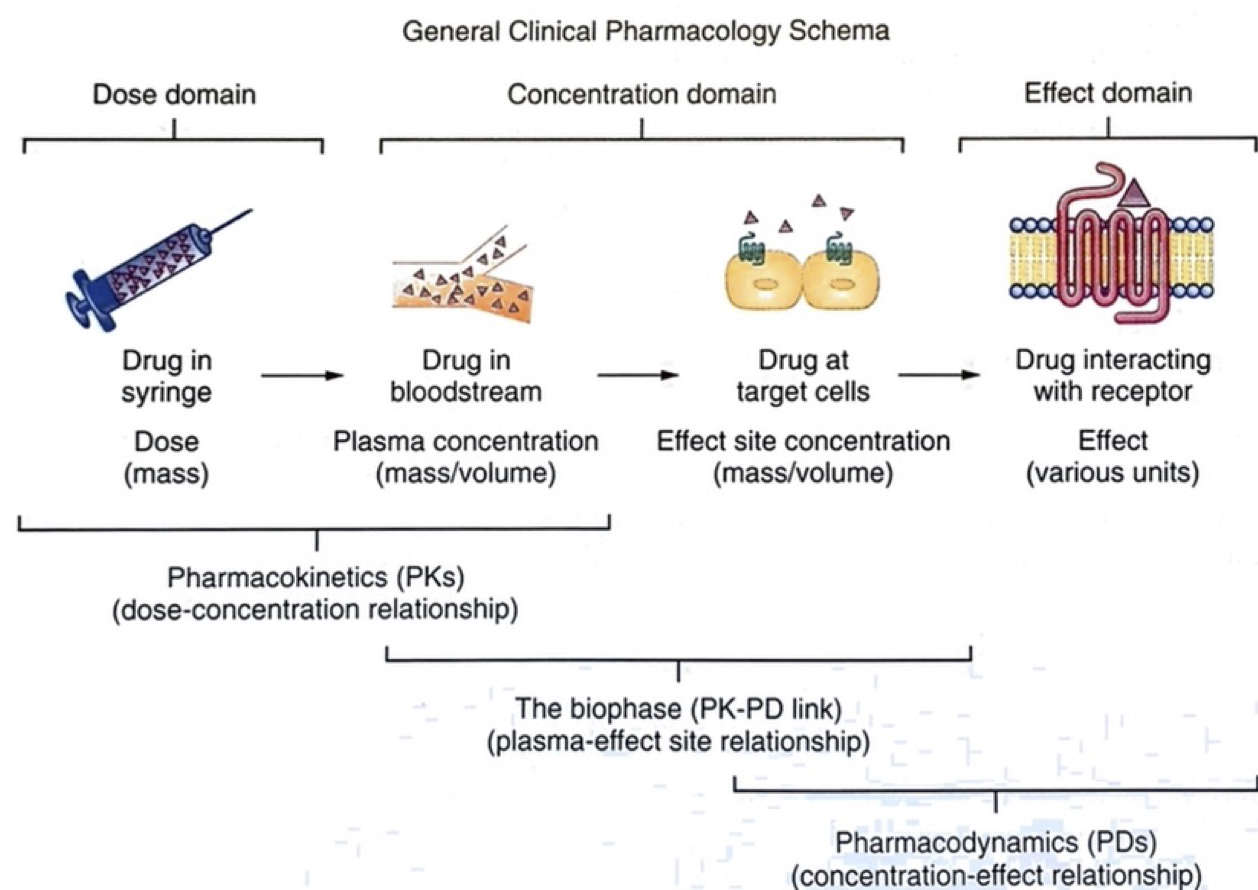
\includegraphics[width=\textheight]{../figures/dose_domains.jpg}
\end{center}
\infina
\end{frame}}

\mode<article>{
\begin{center}
	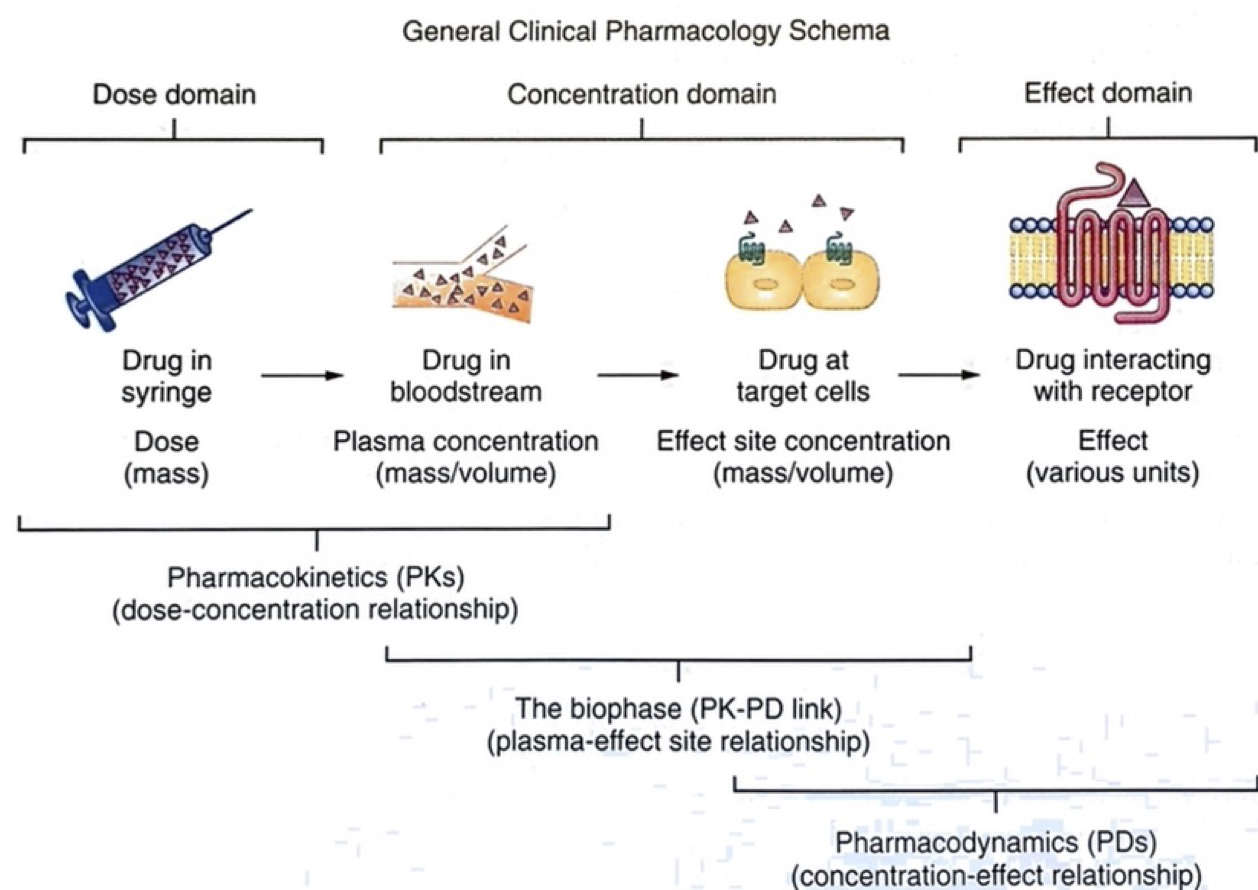
\includegraphics[width=0.6\textwidth]{../figures/dose_domains.jpg}
\end{center}
}


\mode<article>{
	Die Pharmakokinetik und Pharmakodynamik beschreiben zusammen den Prozess von der Applikation (Aufnahme) des Medikamentes bis zur Wirkung. Dies beinhaltet Aufnahme in Blut (bei oraler Applikation), zeitlicher Verlauf der Konzentration im Blut (Umverteilung, Elimination), zeitlicher Verlauf der Aufnahme und Elimination des Medikamentes in den und aus dem Wirkort sowie die Beziehung zwischen der Konzentration am Wirkort und der Wirkung.
}
